\documentclass{ximera}

\input{../../../preamble.tex}


\definecolor{fvdnavy}{HTML}{071D43}
\definecolor{fvdcyan}{HTML}{20BFC6}
\definecolor{fvdcyanlight}{HTML}{EFFCFB}
\definecolor{fvdmagenta}{HTML}{F10D69}
\definecolor{fvdmagentalight}{HTML}{FFF1F7}
\definecolor{fvdtext}{HTML}{163044}





%=================================================
% Pedagogische omgevingen
% PDF: tcolorbox
% HTML: learning-box
%=================================================

\newenvironment{voorkennis}
{%
    \ifdefined\HCode
        \HCode{%
<section class="learning-box learning-box--prior">
<div class="learning-box__header">
<span class="learning-box__icon" aria-hidden="true"></span>
<span class="learning-box__title">Voorkennis</span>
</div>
<div class="learning-box__content">
        }%
        \begin{itemize}
    \else
       \begin{tcolorbox}[
    enhanced,
    breakable,
    colback=fvdcyanlight,
    colframe=fvdcyan,
    coltext=fvdtext,
    boxrule=0.5pt,
    leftrule=4pt,
    arc=4mm,
    outer arc=4mm,
    left=7mm,
    right=6mm,
    top=5mm,
    bottom=5mm,
    before skip=6mm,
    after skip=6mm,
    title=Voorkennis,
    coltitle=fvdcyan,
    fonttitle=\bfseries\Large,
    attach title to upper={\par\smallskip},
    boxed title style={
        empty,
        left=0mm,
        right=0mm,
        top=0mm,
        bottom=0mm
    },
    overlay={
        \draw[
            fvdcyan,
            line width=0.5pt
        ]
        ([xshift=42mm,yshift=-13mm]frame.north west)
        --
        ([xshift=-7mm,yshift=-13mm]frame.north east);
    }
]
        \begin{itemize}
    \fi
}
{%
    \end{itemize}
    \ifdefined\HCode
        \HCode{%
</div>
</section>
        }%
    \else
        \end{tcolorbox}
    \fi
}


\newenvironment{leerdoelen}
{%
    \ifdefined\HCode
        \HCode{%
<section class="learning-box learning-box--goals">
<div class="learning-box__header">
<span class="learning-box__icon" aria-hidden="true"></span>
<span class="learning-box__title">Leerdoelen</span>
</div>
<div class="learning-box__content">
        }%
        \begin{itemize}
    \else
\begin{tcolorbox}[
    enhanced,
    breakable,
    colback=fvdmagentalight,
    colframe=fvdmagenta,
    coltext=fvdtext,
    boxrule=0.5pt,
    leftrule=4pt,
    arc=4mm,
    outer arc=4mm,
    left=7mm,
    right=6mm,
    top=5mm,
    bottom=5mm,
    before skip=6mm,
    after skip=6mm,
    title=Leerdoelen,
    coltitle=fvdmagenta,
    fonttitle=\bfseries\Large,
    attach title to upper={\par\smallskip},
    boxed title style={
        empty,
        left=0mm,
        right=0mm,
        top=0mm,
        bottom=0mm
    },
    overlay={
        \draw[
            fvdmagenta,
            line width=0.5pt
        ]
        ([xshift=42mm,yshift=-13mm]frame.north west)
        --
        ([xshift=-7mm,yshift=-13mm]frame.north east);
    }
]
        \begin{itemize}
    \fi
}
{%
    \end{itemize}
    \ifdefined\HCode
        \HCode{%
</div>
</section>
        }%
    \else
        \end{tcolorbox}
    \fi
}



\title{Primitieve functies van veeltermfuncties}
\author{Ingmar Herreman}

\begin{document}

% FVD_CHAPTER_DATA_START
% Automatisch gegenereerd uit index.tex.
% Niet handmatig aanpassen.
\fvdchapterdata{2}{Van oppervlakte naar integraal}{3}
% FVD_CHAPTER_DATA_END

\begin{abstract}
In het vorige hoofdstuk hebben we de bepaalde integraal opgebouwd als
de limiet van een som van kleine bijdragen. Dat geeft een nauwkeurige
betekenis aan de integraal, maar is geen handige methode om telkens
opnieuw integralen te berekenen.

We zoeken daarom een andere weg. Uit de afgeleidenleer weten we hoe een
functie verandert wanneer we haar afleiden. Nu stellen we de omgekeerde
vraag: als de afgeleide gegeven is, welke oorspronkelijke functie kan
daarbij horen?

Zo komen we bij \textbf{primitieve functies} en bij de
\textbf{onbepaalde integraal}. We concentreren ons eerst op
veeltermfuncties, zodat de basistechniek van het integreren snel en
zeker beheerst wordt.
\end{abstract}

\maketitle

\begin{voorkennis}
  \item Je kan veeltermfuncties afleiden.
  \item Je kent de machtsregel voor afgeleiden.
  \item Je kan sommen, verschillen en constante veelvouden afleiden.
  \item Je kent de betekenis van de bepaalde integraal als limiet van een som en als georiënteerde oppervlakte.
\end{voorkennis}

\begin{leerdoelen}
  \item Je kan uitleggen wat een primitieve functie is.
  \item Je kan aantonen dat primitieve functies van dezelfde functie slechts een constante van elkaar verschillen.
  \item Je begrijpt de betekenis van de integratieconstante \(C\).
  \item Je kan de notatie van de onbepaalde integraal correct lezen en gebruiken.
  \item Je kan de machtsregel voor primitieve functies toepassen.
  \item Je kan primitieve functies van veeltermfuncties bepalen door onmiddellijke integratie en lineariteit.
  \item Je kan een gevonden primitieve controleren door af te leiden.
  \item Je kan uit een bijkomende voorwaarde één specifieke primitieve bepalen.
  \item Je kan foutieve redeneringen en berekeningen bij eenvoudige integralen analyseren.
\end{leerdoelen}

% ============================================================
% 1. DE OMGEKEERDE VRAAG
% ============================================================

\FVDsection{Van afgeleide naar primitieve}

Bij afleiden vertrekken we van een functie en bepalen we haar
afgeleide. Bijvoorbeeld:

\[
F(x)=x^3-2x^2+5x-7
\]

geeft

\[
F'(x)=3x^2-4x+5.
\]

We kunnen ook de omgekeerde vraag stellen:

\begin{center}
\textbf{Welke functie heeft \(3x^2-4x+5\) als afgeleide?}
\end{center}

Eén mogelijk antwoord is

\[
F(x)=x^3-2x^2+5x-7.
\]

Maar ook

\[
G(x)=x^3-2x^2+5x+12
\]

werkt, want

\[
G'(x)=3x^2-4x+5.
\]

De constante term verdwijnt immers bij het afleiden.

\begin{definitie}
Een functie \(F\) heet een \textbf{primitieve functie} van \(f\) op een
interval als

\[
\boxed{F'(x)=f(x)}
\]

voor alle \(x\) in dat interval.
\end{definitie}

\begin{voorbeeld}
Omdat

\[
\left(x^4\right)'=4x^3,
\]

is

\[
F(x)=x^4
\]

een primitieve van

\[
f(x)=4x^3.
\]
\end{voorbeeld}

% ============================================================
% 2. EEN HELE FAMILIE PRIMITIEVEN
% ============================================================

\FVDsection{Een hele familie primitieve functies}

Beschouw

\[
f(x)=3x^2.
\]

Dan zijn onder andere

\[
F_1(x)=x^3,
\]

\[
F_2(x)=x^3+5,
\]

en

\[
F_3(x)=x^3-17
\]

primitieve functies van \(f\), want

\[
F_1'(x)=F_2'(x)=F_3'(x)=3x^2.
\]

De grafieken van deze primitieve functies hebben dezelfde vorm. Ze zijn
alleen verticaal ten opzichte van elkaar verschoven.

\begin{center}
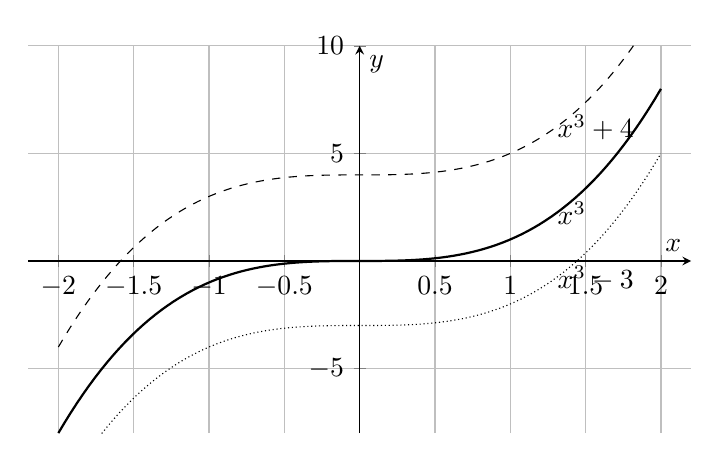
\begin{tikzpicture}
\begin{axis}[
    axis lines=middle,
    xmin=-2.2,xmax=2.2,
    ymin=-8,ymax=10,
    xlabel={$x$},
    ylabel={$y$},
    width=10cm,
    height=6.5cm,
    grid=both
]
    \addplot[black,thick,domain=-2:2,samples=100] {x^3};
    \addplot[black,dashed,domain=-2:2,samples=100] {x^3+4};
    \addplot[black,densely dotted,domain=-2:2,samples=100] {x^3-3};
    \node[anchor=west] at (axis cs:1.25,6.2) {$x^3+4$};
    \node[anchor=west] at (axis cs:1.25,2.2) {$x^3$};
    \node[anchor=west] at (axis cs:1.25,-0.8) {$x^3-3$};
\end{axis}
\end{tikzpicture}
\end{center}

\begin{eigenschap}
Als \(F\) een primitieve functie is van \(f\), dan is voor elke
constante \(C\)

\[
\boxed{F(x)+C}
\]

ook een primitieve functie van \(f\).

Omgekeerd verschillen twee primitieve functies van dezelfde functie op
een interval slechts door een constante.
\end{eigenschap}

Daarom spreken we meestal niet over \emph{de} primitieve, maar over
\emph{een} primitieve of over de volledige familie primitieve functies.

% ============================================================
% 3. ONBEPAALDE INTEGRAAL
% ============================================================

\FVDsection{De onbepaalde integraal}

We gebruiken een compacte notatie voor de volledige familie primitieve
functies.

\begin{definitie}
Als \(F'(x)=f(x)\), dan schrijven we

\[
\boxed{
\int f(x)\,dx=F(x)+C
}
\]

met \(C\in\mathbb{R}\).

Dit noemen we de \textbf{onbepaalde integraal} van \(f\).
\end{definitie}

Bijvoorbeeld:

\[
\int 3x^2\,dx=x^3+C.
\]

In deze notatie noemen we

\begin{itemize}
    \item \(\int\) het integraalteken;
    \item \(f(x)\) de integrand;
    \item \(x\) de integratievariabele;
    \item \(C\) de integratieconstante.
\end{itemize}

\begin{opmerking}
Een \textbf{bepaalde integraal}

\[
\int_a^b f(x)\,dx
\]

is een getal: een georiënteerde accumulatie over het interval
\([a,b]\).

Een \textbf{onbepaalde integraal}

\[
\int f(x)\,dx
\]

beschrijft een familie van primitieve functies.

Dezelfde integraalnotatie wordt dus in twee nauw verwante, maar
verschillende betekenissen gebruikt.
\end{opmerking}

% ============================================================
% 4. INTEGREREN ALS OMGEKEERD AFLIJDEN
% ============================================================

\FVDsection{Integreren als omgekeerd afleiden}

Voor veeltermfuncties kunnen we de integratieregels rechtstreeks uit de
afleidingsregels afleiden.

We weten:

\[
\left(x^{n+1}\right)'=(n+1)x^n.
\]

Om bij het afleiden precies \(x^n\) over te houden, delen we door
\(n+1\):

\[
\left(\frac{x^{n+1}}{n+1}\right)'=x^n.
\]

Daaruit volgt de belangrijkste basisregel.

\begin{eigenschap}[Machtsregel]
Voor \(n\neq -1\):

\[
\boxed{
\int x^n\,dx
=
\frac{x^{n+1}}{n+1}+C
}
\]
\end{eigenschap}

Voor veeltermen gebruiken we voorlopig vooral

\[
n=0,1,2,3,\ldots
\]

\begin{voorbeeld}
\[
\int x^4\,dx
=
\frac{x^5}{5}+C.
\]

Controle:

\[
\left(\frac{x^5}{5}+C\right)'
=
x^4.
\]
\end{voorbeeld}

\begin{opmerking}
Bij integreren met de machtsregel:

\[
\boxed{
\text{exponent één verhogen}
\quad\text{en vervolgens delen door de nieuwe exponent}
}
\]

Dit is precies de omgekeerde beweging van de machtsregel voor
afgeleiden.
\end{opmerking}

% ============================================================
% 5. CONSTANTE FUNCTIES
% ============================================================

\FVDsection{Constante functies}

Een constante functie kunnen we schrijven als

\[
k=kx^0.
\]

Met de machtsregel:

\[
\int k\,dx
=
k\frac{x^1}{1}+C.
\]

Dus:

\begin{eigenschap}
Voor elke constante \(k\):

\[
\boxed{
\int k\,dx=kx+C.
}
\]
\end{eigenschap}

\begin{voorbeeld}
\[
\int 7\,dx=7x+C.
\]
\end{voorbeeld}

Dit is ook onmiddellijk te controleren:

\[
(7x+C)'=7.
\]

% ============================================================
% 6. LINEARITEIT
% ============================================================

\FVDsection{Sommen, verschillen en constante factoren}

Net zoals bij afleiden kunnen we veeltermen term voor term behandelen.

\begin{eigenschap}[Lineariteit]
Voor integreerbare functies \(f\) en \(g\) en een constante
\(\lambda\) geldt:

\[
\int\left(f(x)+g(x)\right)\,dx
=
\int f(x)\,dx+\int g(x)\,dx,
\]

\[
\int\left(f(x)-g(x)\right)\,dx
=
\int f(x)\,dx-\int g(x)\,dx,
\]

en

\[
\int \lambda f(x)\,dx
=
\lambda\int f(x)\,dx.
\]
\end{eigenschap}

Daardoor kunnen we een veelterm \textbf{term voor term integreren}.

\begin{voorbeeld}
Bereken

\[
\int(3x^2-4x+5)\,dx.
\]

We splitsen:

\[
\int(3x^2-4x+5)\,dx
=
3\int x^2\,dx
-
4\int x\,dx
+
5\int1\,dx.
\]

Dus

\[
=
3\frac{x^3}{3}
-
4\frac{x^2}{2}
+
5x+C.
\]

Na vereenvoudigen:

\[
\boxed{
\int(3x^2-4x+5)\,dx
=
x^3-2x^2+5x+C.
}
\]
\end{voorbeeld}

\begin{opmerking}
Bij één onbepaalde integraal schrijven we uiteindelijk slechts
\textbf{één} integratieconstante \(C\).

Je zou tijdens het splitsen verschillende constanten kunnen schrijven,
maar hun som of verschil is opnieuw één willekeurige constante.
\end{opmerking}

% ============================================================
% 7. EEN VASTE WERKWIJZE
% ============================================================

\FVDsection{Veeltermfuncties systematisch integreren}

Voor veeltermfuncties is de volgende werkwijze betrouwbaar.

\begin{enumerate}
    \item Schrijf de veelterm als een som of verschil van afzonderlijke termen.
    \item Neem constante factoren mee naar buiten.
    \item Verhoog bij elke macht van \(x\) de exponent met \(1\).
    \item Deel door die nieuwe exponent.
    \item Vereenvoudig.
    \item Voeg \(+C\) toe.
    \item Controleer indien nodig door het antwoord af te leiden.
\end{enumerate}

\begin{voorbeeld}
Bepaal

\[
\int(6x^5-3x^2+8x-4)\,dx.
\]

Term voor term:

\[
\int6x^5\,dx=x^6,
\]

\[
\int(-3x^2)\,dx=-x^3,
\]

\[
\int8x\,dx=4x^2,
\]

en

\[
\int(-4)\,dx=-4x.
\]

Dus

\[
\boxed{
\int(6x^5-3x^2+8x-4)\,dx
=
x^6-x^3+4x^2-4x+C.
}
\]

Controle:

\[
\left(x^6-x^3+4x^2-4x+C\right)'
=
6x^5-3x^2+8x-4.
\]
\end{voorbeeld}

% ============================================================
% 8. EERST VEREENVOUDIGEN
% ============================================================

\FVDsection{Eerst algebra, dan integreren}

Niet elke veelterm staat onmiddellijk in een handige vorm. Soms moeten
we eerst haakjes wegwerken of gelijksoortige termen samennemen.

\begin{voorbeeld}
Bereken

\[
\int\left(2x(x^2-3)+x^3+4\right)\,dx.
\]

Eerst vereenvoudigen:

\[
2x(x^2-3)+x^3+4
=
2x^3-6x+x^3+4
=
3x^3-6x+4.
\]

Daarna integreren:

\[
\int(3x^3-6x+4)\,dx
=
\frac34x^4-3x^2+4x+C.
\]

Dus

\[
\boxed{
\int\left(2x(x^2-3)+x^3+4\right)\,dx
=
\frac34x^4-3x^2+4x+C.
}
\]
\end{voorbeeld}

\begin{opmerking}
Integreren is geen vervanging voor algebra. Een uitdrukking eerst
herkennen en vereenvoudigen kan de integratie veel eenvoudiger maken.
\end{opmerking}

% ============================================================
% 9. CONTROLEREN DOOR AF TE LEIDEN
% ============================================================

\FVDsection{Je antwoord controleren}

Omdat integreren hier het omgekeerde proces van afleiden is, hebben we
een bijzonder eenvoudige controle.

Als je beweert dat

\[
\int f(x)\,dx=F(x)+C,
\]

dan moet

\[
F'(x)=f(x).
\]

\begin{voorbeeld}[Een fout opsporen]

Een leerling schrijft:

\[
\int 4x^3\,dx=4x^4+C.
\]

We leiden het voorgestelde antwoord af:

\[
(4x^4+C)'=16x^3.
\]

Dat is niet de oorspronkelijke integrand \(4x^3\). Het antwoord is dus
fout.

Correct is:

\[
\int4x^3\,dx
=
4\frac{x^4}{4}+C
=
x^4+C.
\]
\end{voorbeeld}

\begin{opmerking}
Maak van deze controle een gewoonte, zeker wanneer je twijfelt over een
coëfficiënt of exponent.
\end{opmerking}

% ============================================================
% 10. DE INTEGRATIECONSTANTE IS ESSENTIEEL
% ============================================================

\FVDsection{Waarom \(+C\) niet mag ontbreken}

Een veelgemaakte fout is

\[
\int 2x\,dx=x^2.
\]

De functie \(x^2\) is inderdaad \emph{een} primitieve van \(2x\), maar
de onbepaalde integraal vraagt naar de volledige familie.

Daarom:

\[
\boxed{
\int2x\,dx=x^2+C.
}
\]

\begin{voorbeeld}
Welke van de volgende functies zijn primitieve functies van
\(f(x)=6x-2\)?

\[
F(x)=3x^2-2x,
\]

\[
G(x)=3x^2-2x+11,
\]

\[
H(x)=3x^2-2x-\pi.
\]

We vinden:

\[
F'(x)=G'(x)=H'(x)=6x-2.
\]

Ze zijn dus alle drie primitieve functies van \(f\).

Daarom vatten we ze samen als

\[
\int(6x-2)\,dx
=
3x^2-2x+C.
\]
\end{voorbeeld}

% ============================================================
% 11. EEN SPECIFIEKE PRIMITIEVE
% ============================================================

\FVDsection{Een primitieve bepalen met een voorwaarde}

De integratieconstante \(C\) betekent dat er oneindig veel primitieve
functies zijn.

Een bijkomende voorwaarde kan precies één lid van die familie
selecteren.

\begin{voorbeeld}
Bepaal de primitieve functie \(F\) van

\[
f(x)=6x^2-4x+3
\]

waarvoor

\[
F(1)=5.
\]

Eerst bepalen we de volledige familie:

\[
F(x)
=
2x^3-2x^2+3x+C.
\]

Nu gebruiken we \(F(1)=5\):

\[
2-2+3+C=5.
\]

Dus

\[
3+C=5
\]

en bijgevolg

\[
C=2.
\]

De gevraagde primitieve is

\[
\boxed{
F(x)=2x^3-2x^2+3x+2.
}
\]
\end{voorbeeld}

Dit principe zal later belangrijk worden wanneer een beginwaarde of
andere voorwaarde gegeven is.

% ============================================================
% 12. GRAFISCH DENKEN
% ============================================================

\FVDsection{Wat vertelt \(f\) over haar primitieve?}

Als \(F\) een primitieve is van \(f\), dan

\[
F'(x)=f(x).
\]

Alles wat we over het teken van een afgeleide geleerd hebben, kunnen we
dus opnieuw gebruiken.

\begin{itemize}
    \item Als \(f(x)>0\), dan is \(F'(x)>0\) en is \(F\) stijgend.
    \item Als \(f(x)<0\), dan is \(F'(x)<0\) en is \(F\) dalend.
    \item Als \(f(x)=0\), dan heeft \(F\) daar een horizontale raaklijn.
\end{itemize}

\begin{voorbeeld}
Stel dat

\[
f(x)=x^2-1.
\]

De nulpunten zijn

\[
x=-1
\qquad\text{en}\qquad
x=1.
\]

Verder:

\[
f(x)>0
\quad\text{voor}\quad
x<-1\ \text{of}\ x>1,
\]

en

\[
f(x)<0
\quad\text{voor}\quad
-1<x<1.
\]

Elke primitieve \(F\) van \(f\) is dus stijgend op

\[
]-\infty,-1[
\quad\text{en}\quad
]1,+\infty[
\]

en dalend op

\[
]-1,1[.
\]

We kunnen dit besluiten zonder eerst een formule voor \(F\) te
berekenen.
\end{voorbeeld}

\begin{opmerking}
Dit soort redenering is belangrijk: integreren is niet alleen een
rekenprocedure. De relatie

\[
F'=f
\]

laat ons ook functies analyseren.
\end{opmerking}

% ============================================================
% 13. BEPAALDE EN ONBEPAALDE INTEGRAAL KOMEN SAMEN
% ============================================================

\FVDsection{Twee ideeën die nog verbonden moeten worden}

We beschikken nu over twee verschillende inzichten.

Uit het vorige hoofdstuk kennen we de bepaalde integraal

\[
\int_a^b f(x)\,dx,
\]

die een georiënteerde accumulatie voorstelt en als limiet van
Riemannsommen werd gedefinieerd.

In dit hoofdstuk leerden we primitieve functies bepalen:

\[
\int f(x)\,dx=F(x)+C.
\]

Voor bijvoorbeeld

\[
f(x)=3x^2-4x+2
\]

vinden we onmiddellijk

\[
F(x)=x^3-2x^2+2x+C.
\]

Maar daarmee blijft één fundamentele vraag open:

\begin{center}
\textbf{Kan een primitieve functie ons helpen om de bepaalde integraal
\(\displaystyle\int_a^b f(x)\,dx\) snel te berekenen?}
\end{center}

Als het antwoord ja is, hoeven we niet telkens opnieuw Riemannsommen en
limieten uit te werken.

Het verband tussen beide ideeën is een van de centrale resultaten van
de integraalrekening. Dat onderzoeken we in het volgende hoofdstuk.

\end{document}
